\documentclass[12pt]{beamer}
\usepackage[english, russian]{babel}
\usepackage[utf8]{inputenc}
\usepackage{graphicx}
\usepackage{hyperref}
\usepackage{minted}
\usepackage{amsmath}
\usepackage{amssymb}

\graphicspath{
    {assets},
    {assets/erd},
    {assets/logo},
    {assets/misc},
    {assets/uf},
    {assets/screenshots}
}

\usetheme{Madrid}

\title[Сайт для аренды вещей]
{Разработка клиент-серверного приложения для аренды вещей}
\author[Карабалин Руслан]{Выполнил: Карабалин Руслан}
\institute[ОмГУ]
{
    ОмГУ им. Ф.М. Достоевского \\
    \vspace{0.5cm}
    Научный руководитель: канд.физ.-мат.наук Ашаева Юлия Михайловна \\
    \vspace{0.5cm}
}
\date{}

\begin{document}
	
	\begin{frame}
            \begin{columns}

                \column{0.6\textwidth}
    
                \column{0.4\textwidth}
                
\includegraphics[width=1\textwidth]{omsu.png}
            
            \end{columns}
    
		\titlepage
	\end{frame}

    \section{Проблема}
    \begin{frame}
        \frametitle{Проблема}

        \begin{center}
            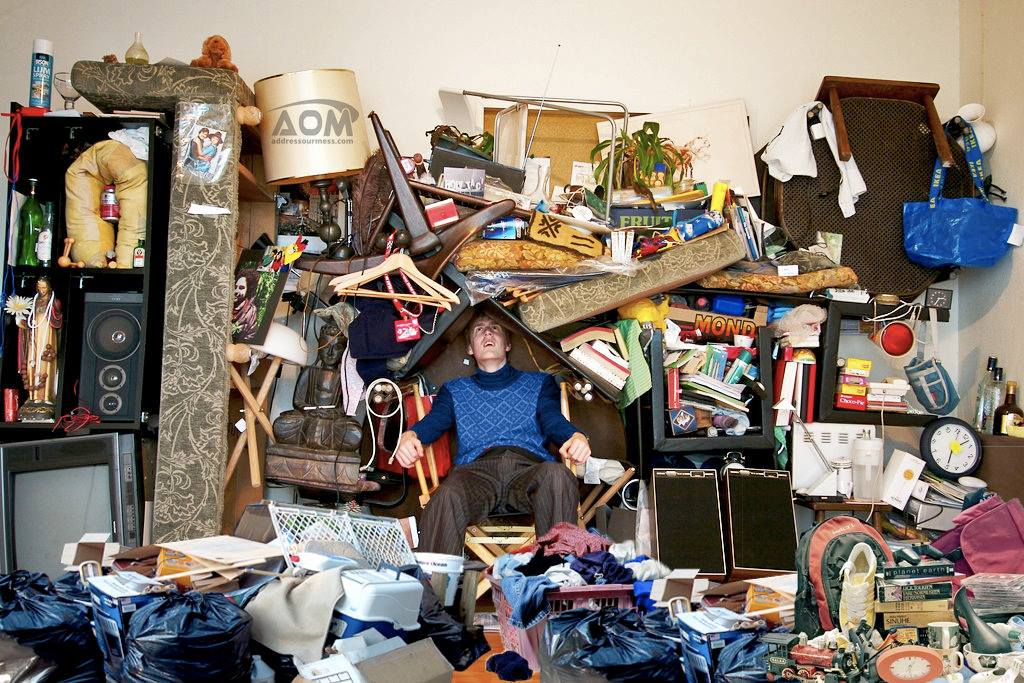
\includegraphics[width=0.8\textwidth]{room.jpg}
        \end{center}

    \end{frame}

    \section{Цель}
    \begin{frame}
        \frametitle{Цель}

        \begin{center}
        
            Разработать веб-приложение для аренды вещей.
            
            \vspace{0.5cm}
            
            
\includegraphics[width=0.7\textwidth]{web-site.jpg}
            
        \end{center}
        
    \end{frame}

    \section{Задачи}
    \begin{frame}
        \frametitle{Задачи}

        \begin{columns}

            \column{0.6\textwidth}
            \begin{itemize}
                \item Формирование концепции
                \item Определение требований
                \item Разработка схемы базы данных
                \item Создание серверной части
                \item Создание клиентской части
            \end{itemize}

            \column{0.4\textwidth}
            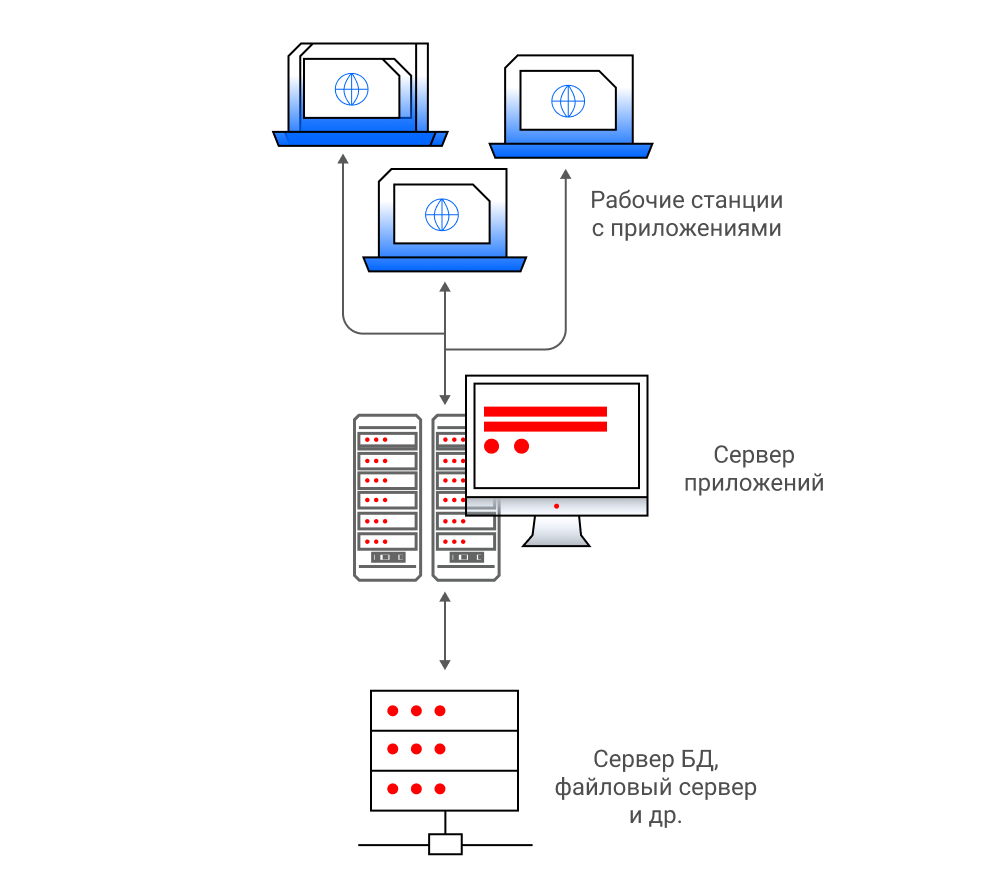
\includegraphics[width=1\textwidth]{arch.png}
            
        \end{columns}
        
    \end{frame}

    \section{Средства решения}
    \begin{frame}
        \frametitle{Средства решения}

        \vspace{-1cm}

        \begin{columns}

            \column{0.4\textwidth}
            \begin{itemize}
                \item Клиентская часть
                \begin{itemize}
                    \item React
                    \item Redux
                \end{itemize}
                \item Серверная часть
                \begin{itemize}
                    \item Kotlin
                    \item Spring Boot
                \end{itemize}
                \item Хранилища данных
                \begin{itemize}
                    \item PostgreSQL
                    \item Yandex Object Storage
                \end{itemize}
            \end{itemize}

            \column{0.6\textwidth}
            \begin{center}
                
\includegraphics[width=0.2\textwidth]{react.png}
                \vspace{0.5cm}
                
\includegraphics[width=0.2\textwidth]{redux.png}
                \vspace{0.5cm}
                
                
\includegraphics[width=0.2\textwidth]{kotlin.png}
                \vspace{0.5cm}
                
\includegraphics[width=0.2\textwidth]{spring.png}
                \vspace{0.5cm}
                
                
\includegraphics[width=0.2\textwidth]{postgresql.png}
            \end{center}
            
        \end{columns}
        
    \end{frame}

    \section{Основная функциональность}
    \begin{frame}
    \frametitle{Основная функциональность}

        \vspace{-1cm}

        \begin{itemize}
            \item Регистрация
            \item Создание объявлений
            \item Поиск объявлений
            \item Аренда вещи из объявления
            \newline
        \end{itemize}

        Сервис позволит пользователям находить нужные вещи и
        самостоятельно связываться друг с другом.
    \end{frame}

    \section{Сценарий взаимодействия}
    \begin{frame}
    \frametitle{Сценарий взаимодействия}
        \begin{center}
            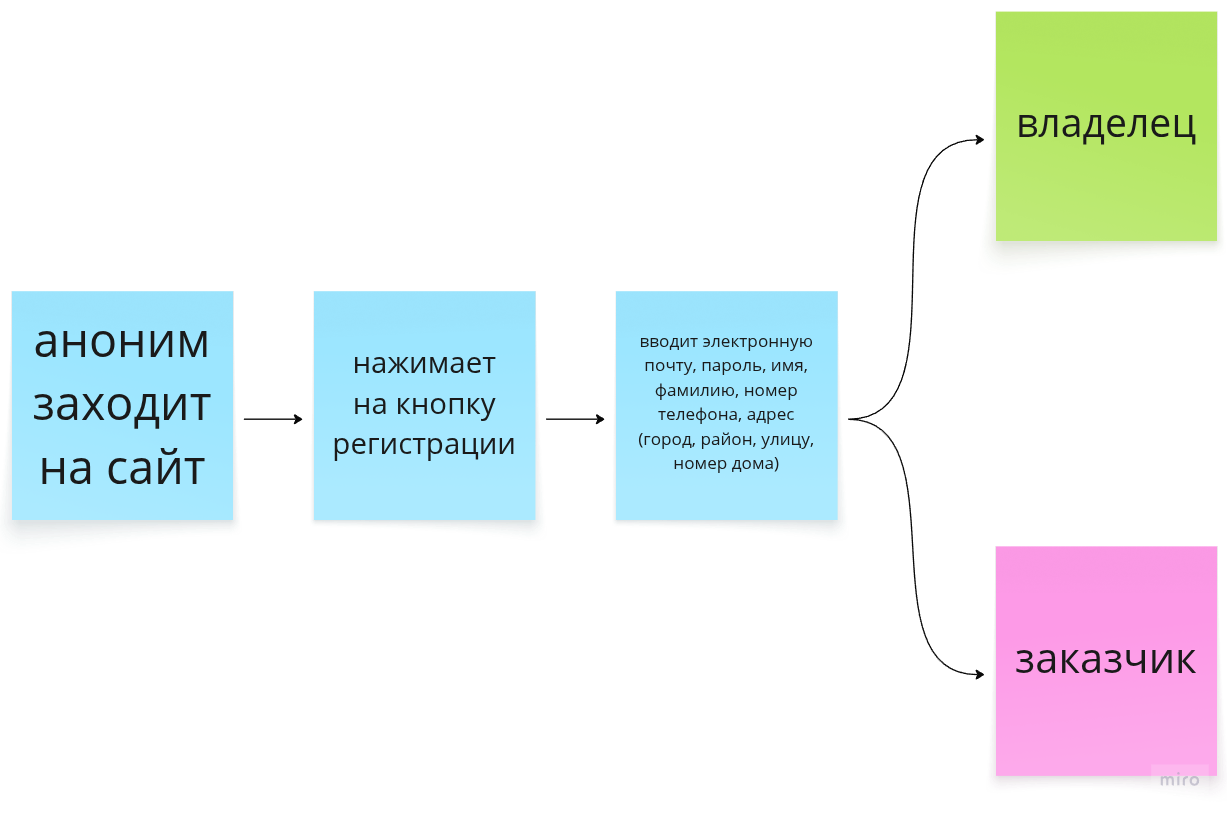
\includegraphics[width=1\textwidth]{uf01.png}
        \end{center}        
    \end{frame}

    \begin{frame}
    \frametitle{Сценарий взаимодействия}
        \begin{center}
            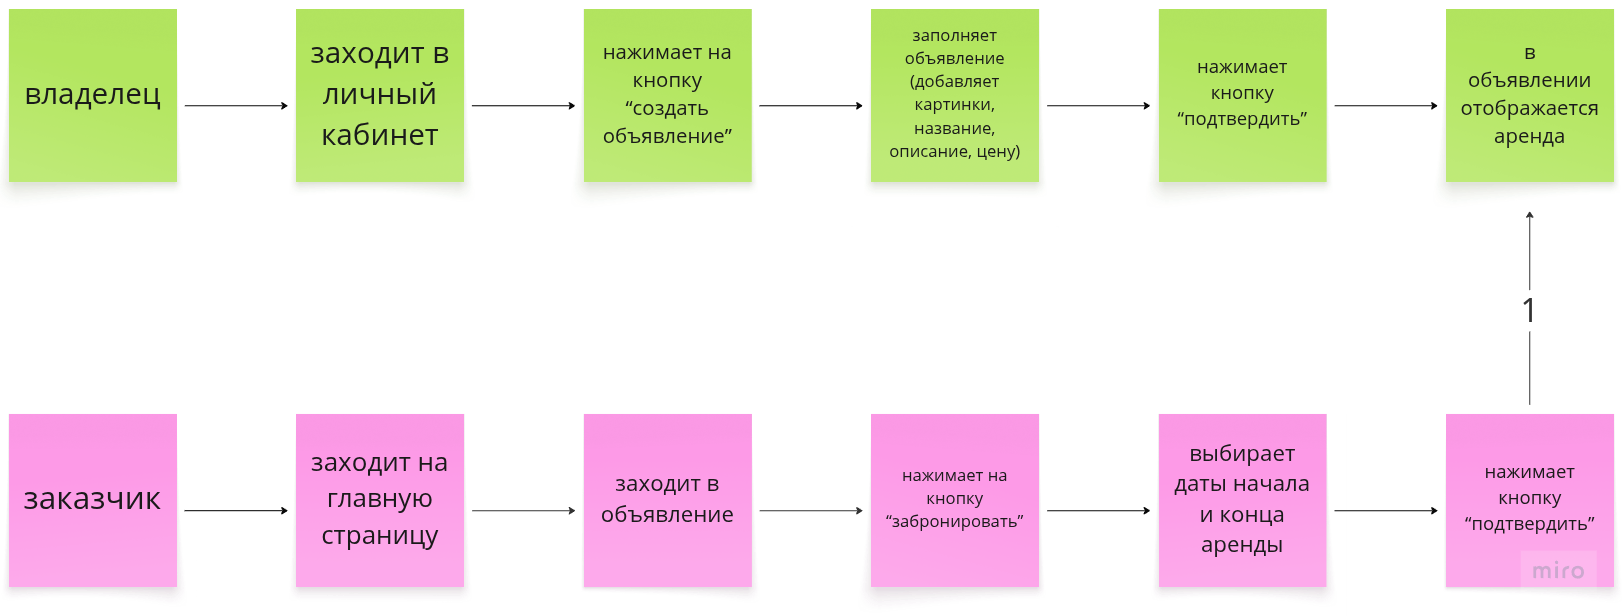
\includegraphics[width=1\textwidth]{uf02.png}
        \end{center}
    \end{frame}

    \begin{frame}
    \frametitle{Сценарий взаимодействия}
        \begin{center}
            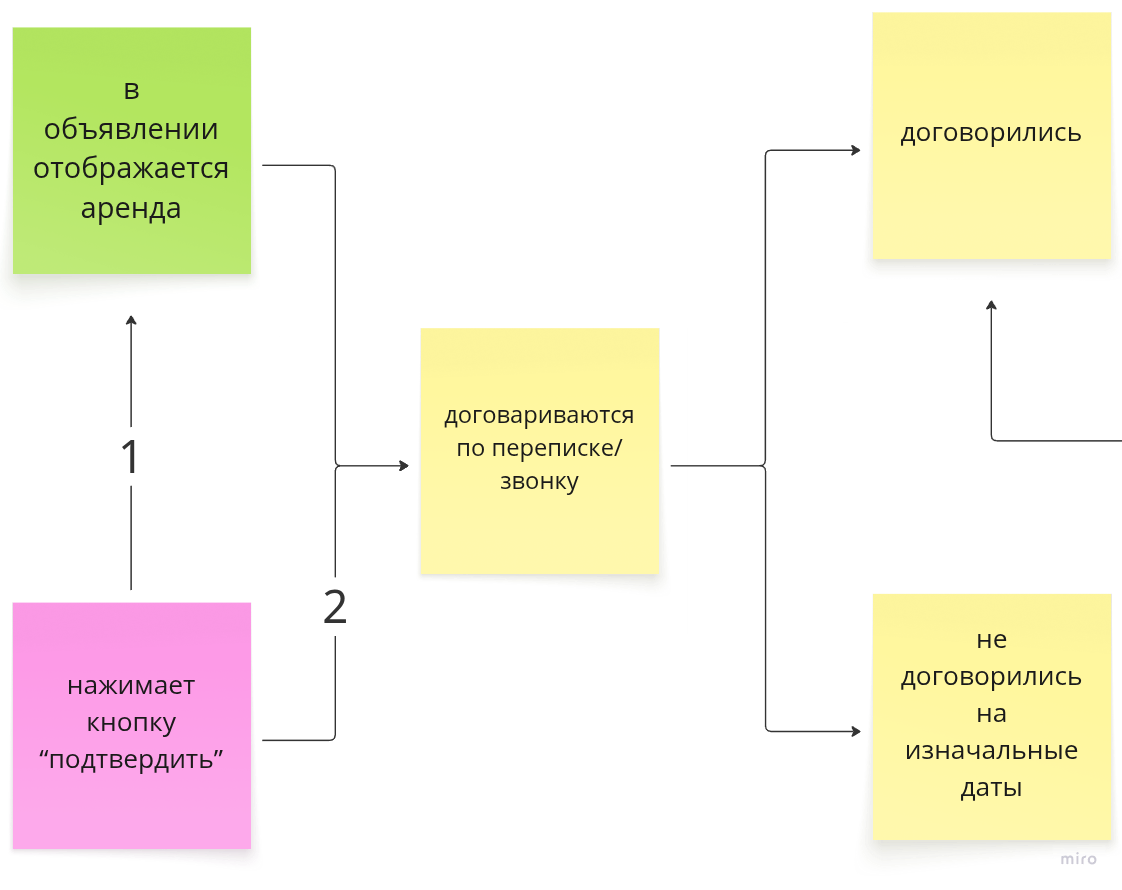
\includegraphics[width=0.8\textwidth]{uf03.png}
        \end{center}
    \end{frame}

    \begin{frame}
    \frametitle{Сценарий взаимодействия}
        \begin{center}
            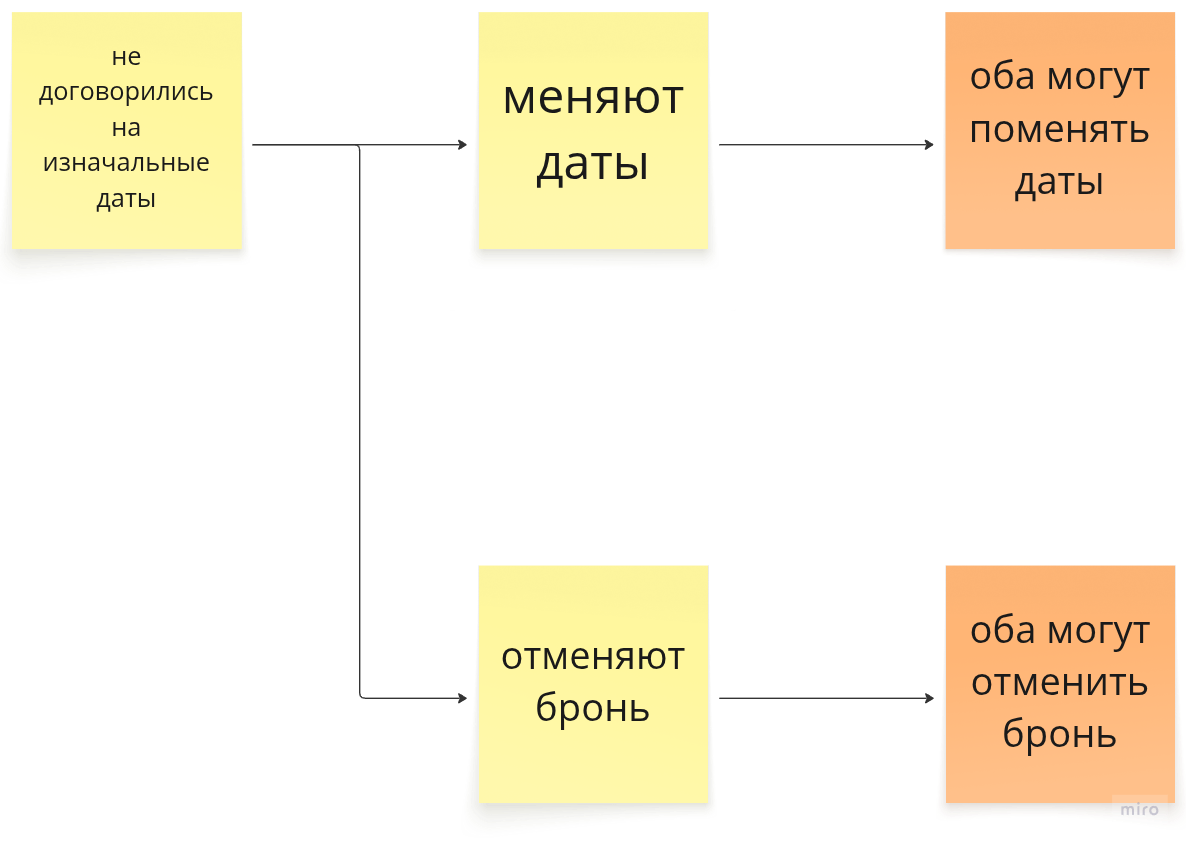
\includegraphics[width=0.9\textwidth]{uf04.png}
        \end{center}
    \end{frame}

    \begin{frame}
    \frametitle{Сценарий взаимодействия}
        \begin{center}
            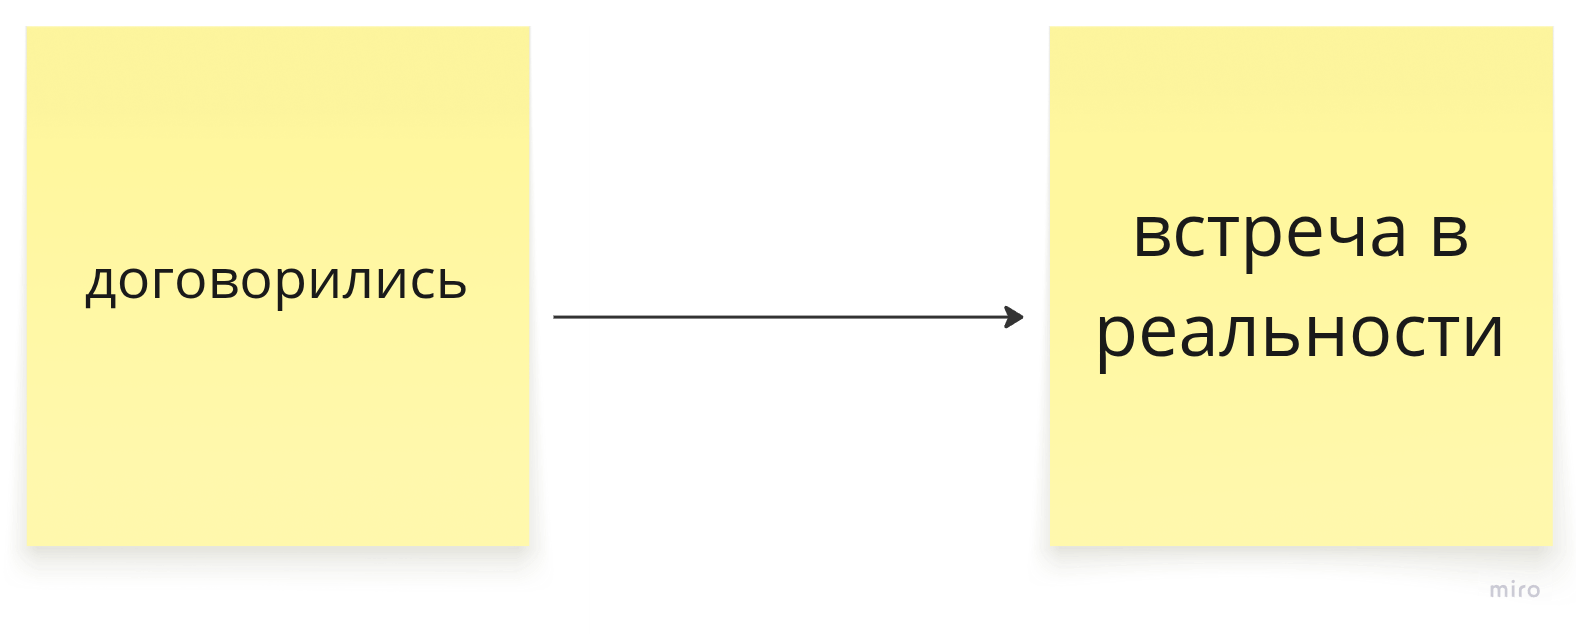
\includegraphics[width=0.8\textwidth]{uf05.png}
        \end{center}
    \end{frame}

    \section{Схема базы данных}
    \begin{frame}
    \frametitle{Схема базы данных}
        \begin{center}
            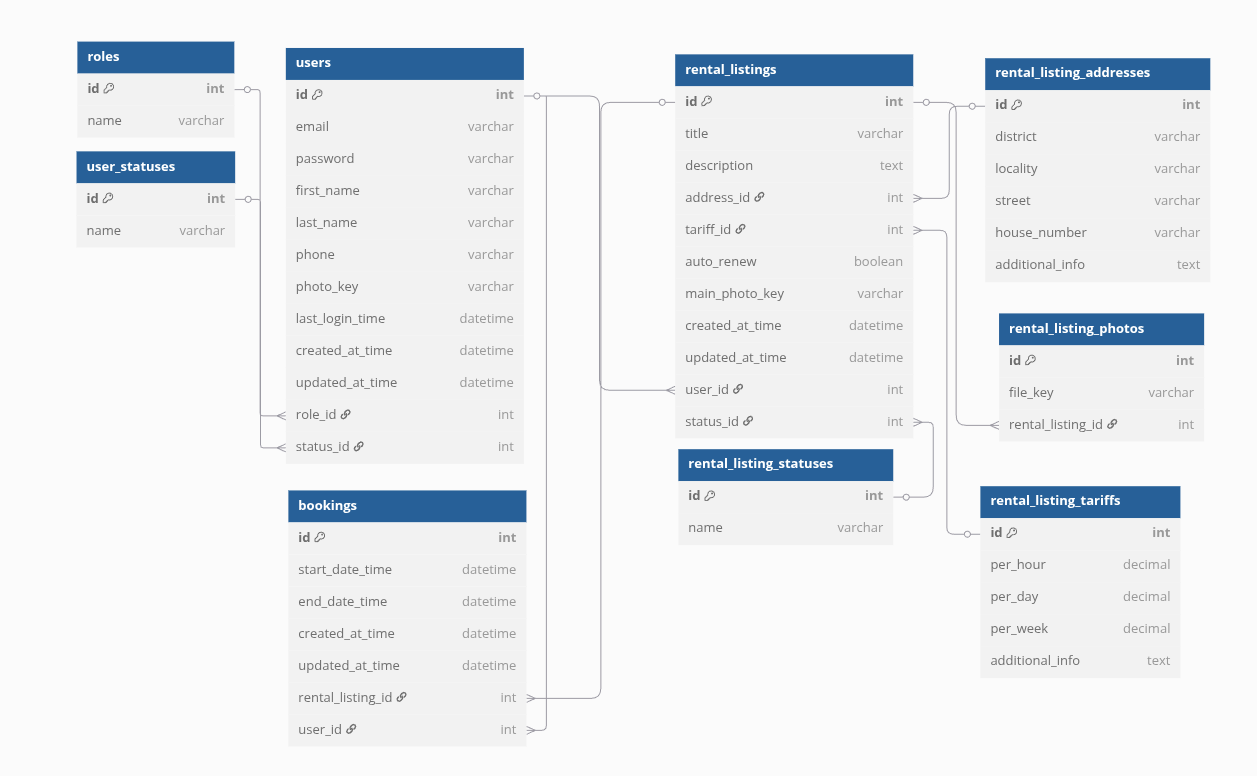
\includegraphics[width=1.0\textwidth]{erd.png}
        \end{center}
    \end{frame}

{
    \definecolor{myBlue}{rgb}{0.7, 1.0, 0.7}
    \setbeamercolor{background canvas}{bg=myBlue}
    
    \section{Демонстрация работы приложения}
    \begin{frame}
    \frametitle{Демонстрация работы приложения}
        \begin{center}
            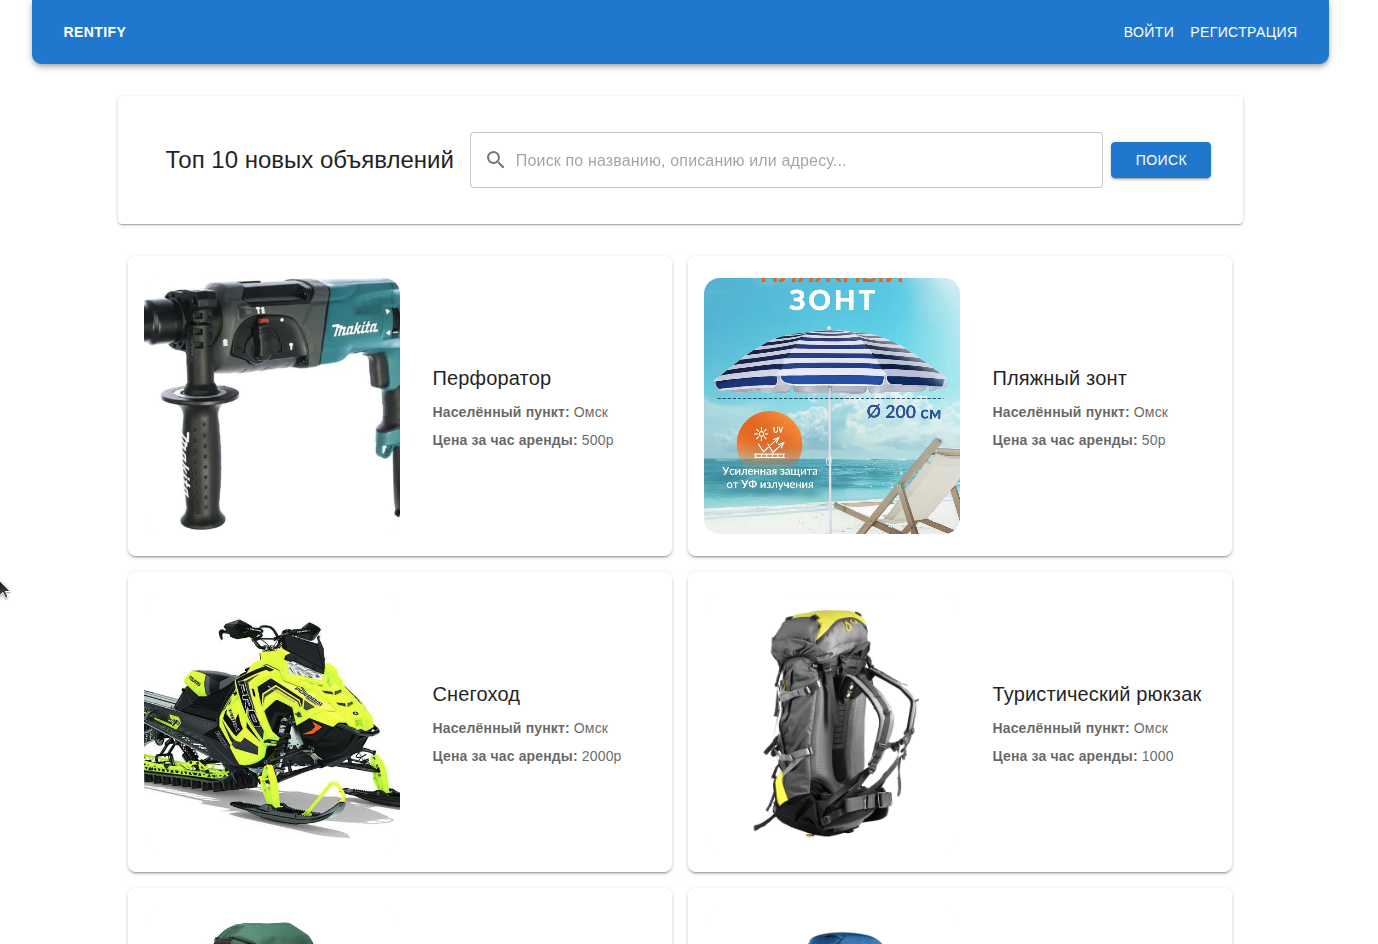
\includegraphics[width=0.9\textwidth]{homePage.png}
        \end{center}
    \end{frame}

    \begin{frame}
        \begin{center}
            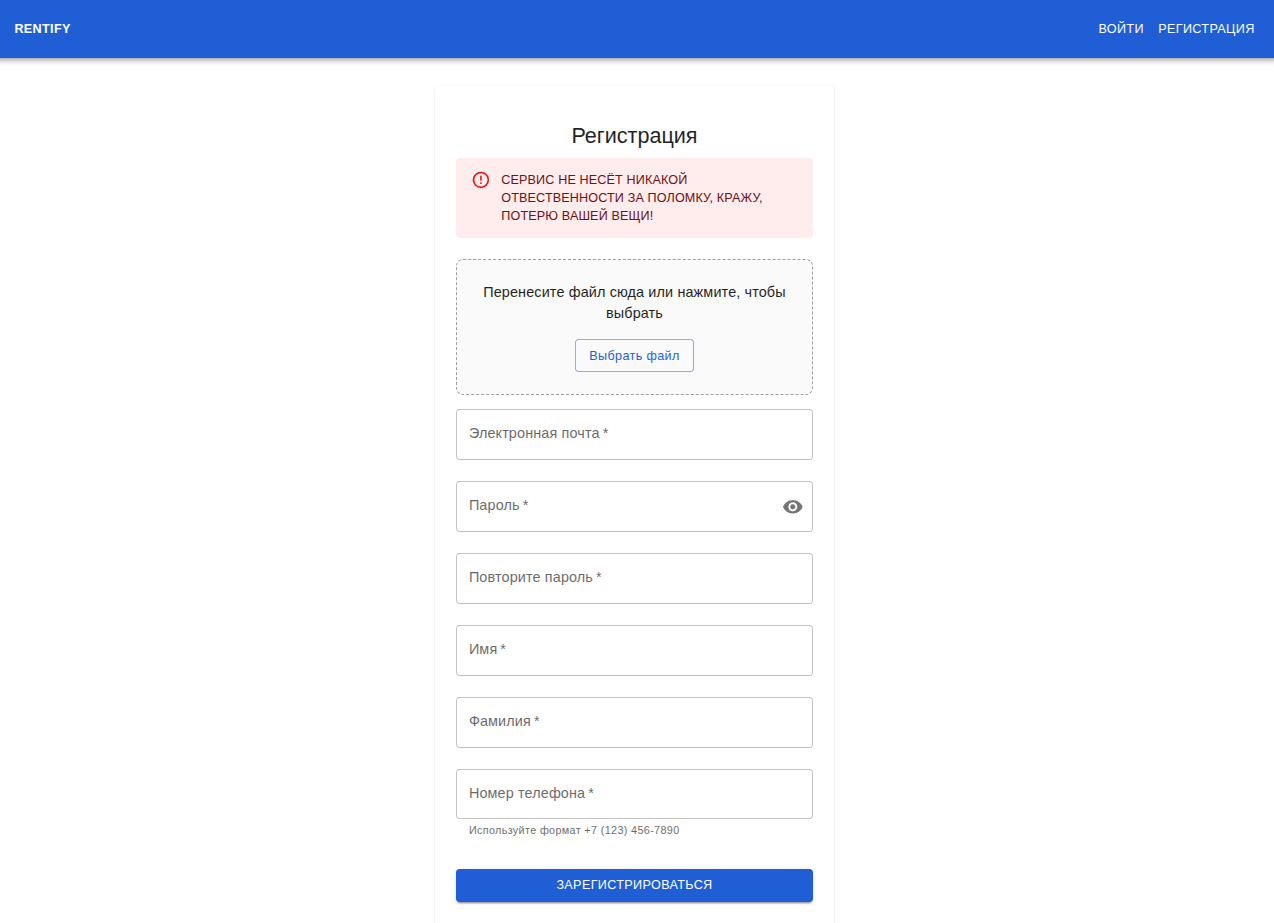
\includegraphics[width=1\textwidth]{register.png}
        \end{center}
    \end{frame}

    \begin{frame}
        \begin{center}
            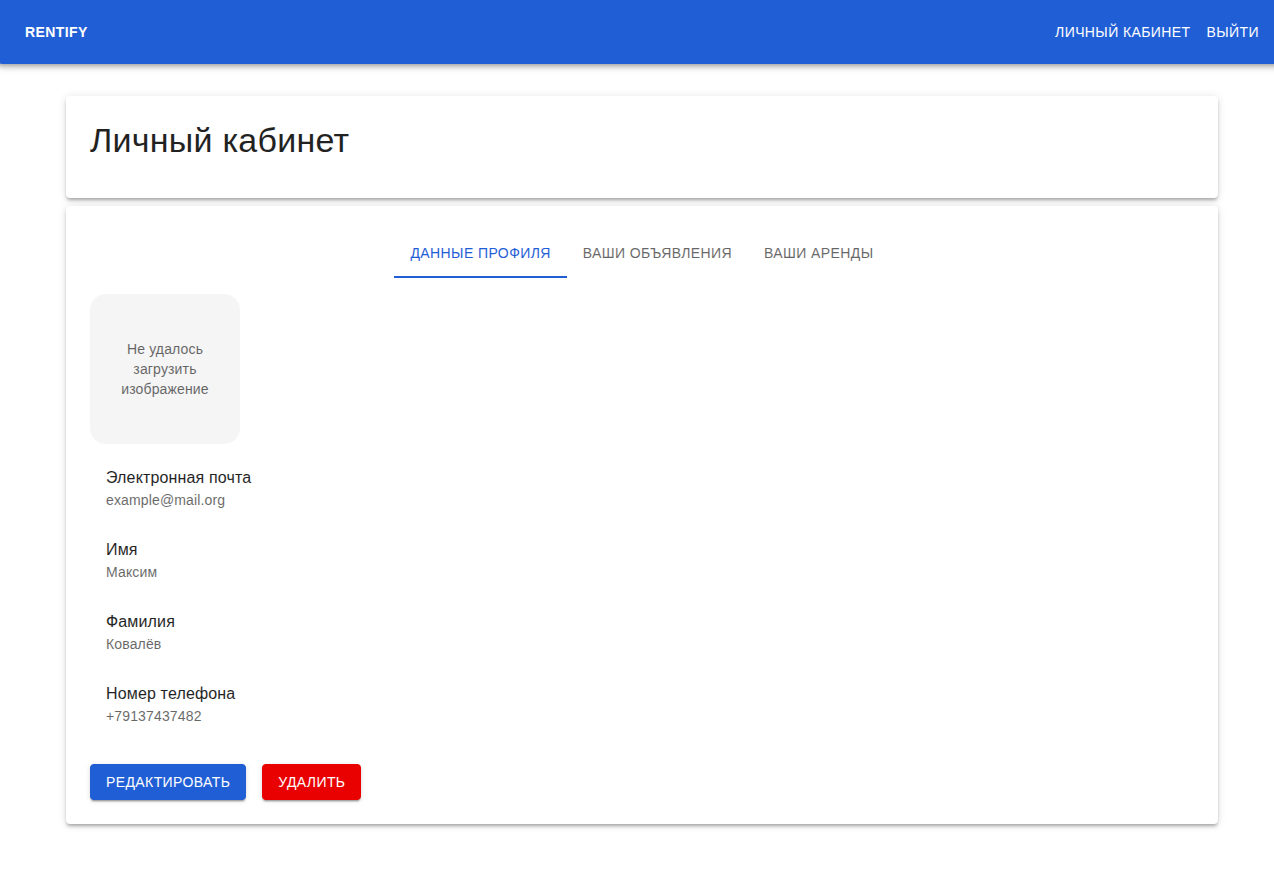
\includegraphics[width=1\textwidth]{account.png}
        \end{center}
    \end{frame}

    \begin{frame}
        \begin{center}
            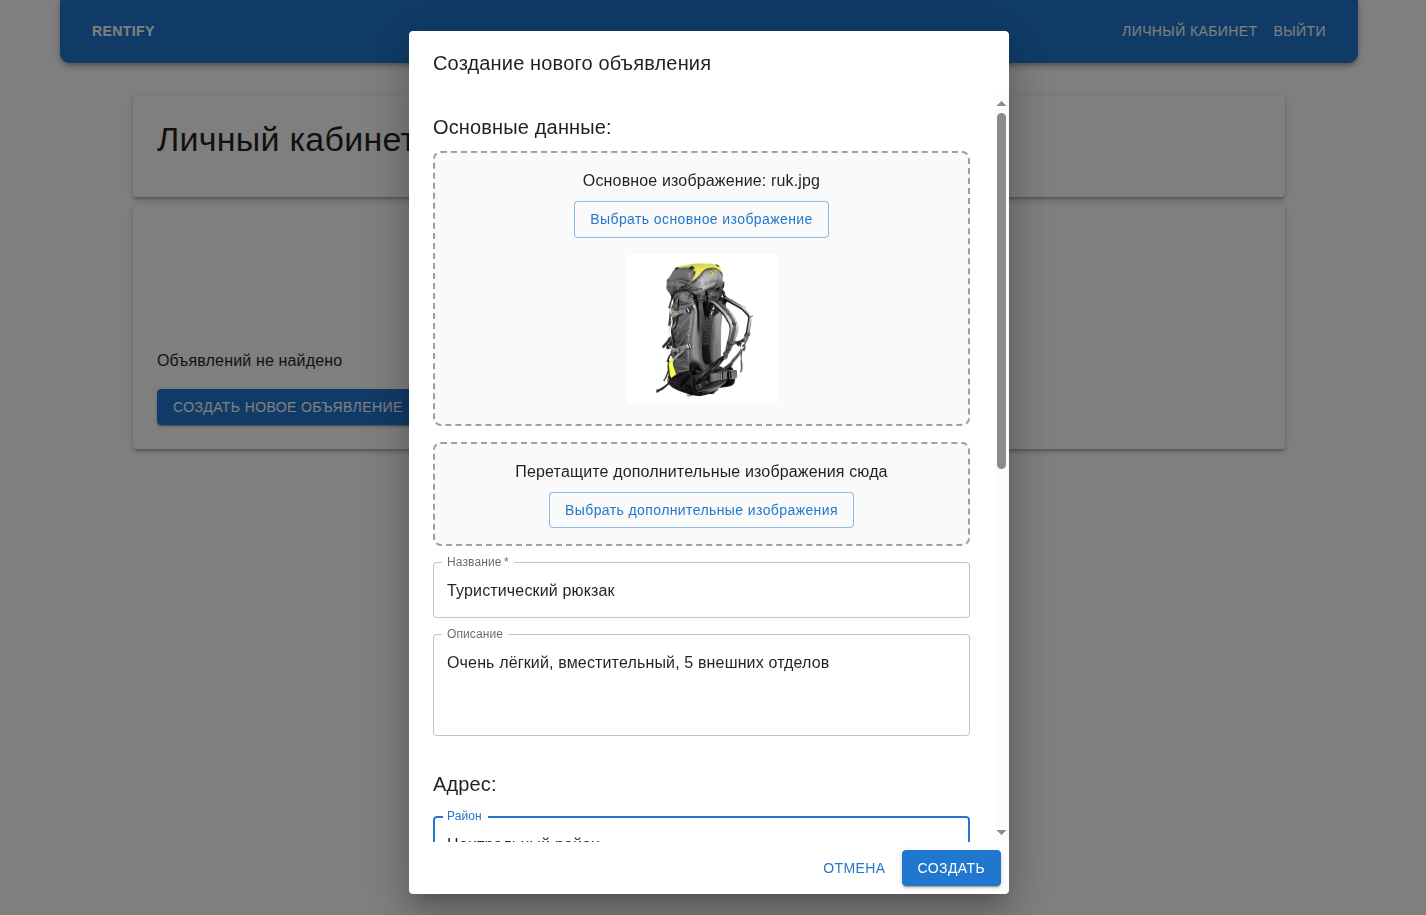
\includegraphics[width=1\textwidth]{listing01.png}
        \end{center}
    \end{frame}

    \begin{frame}
        \begin{center}
            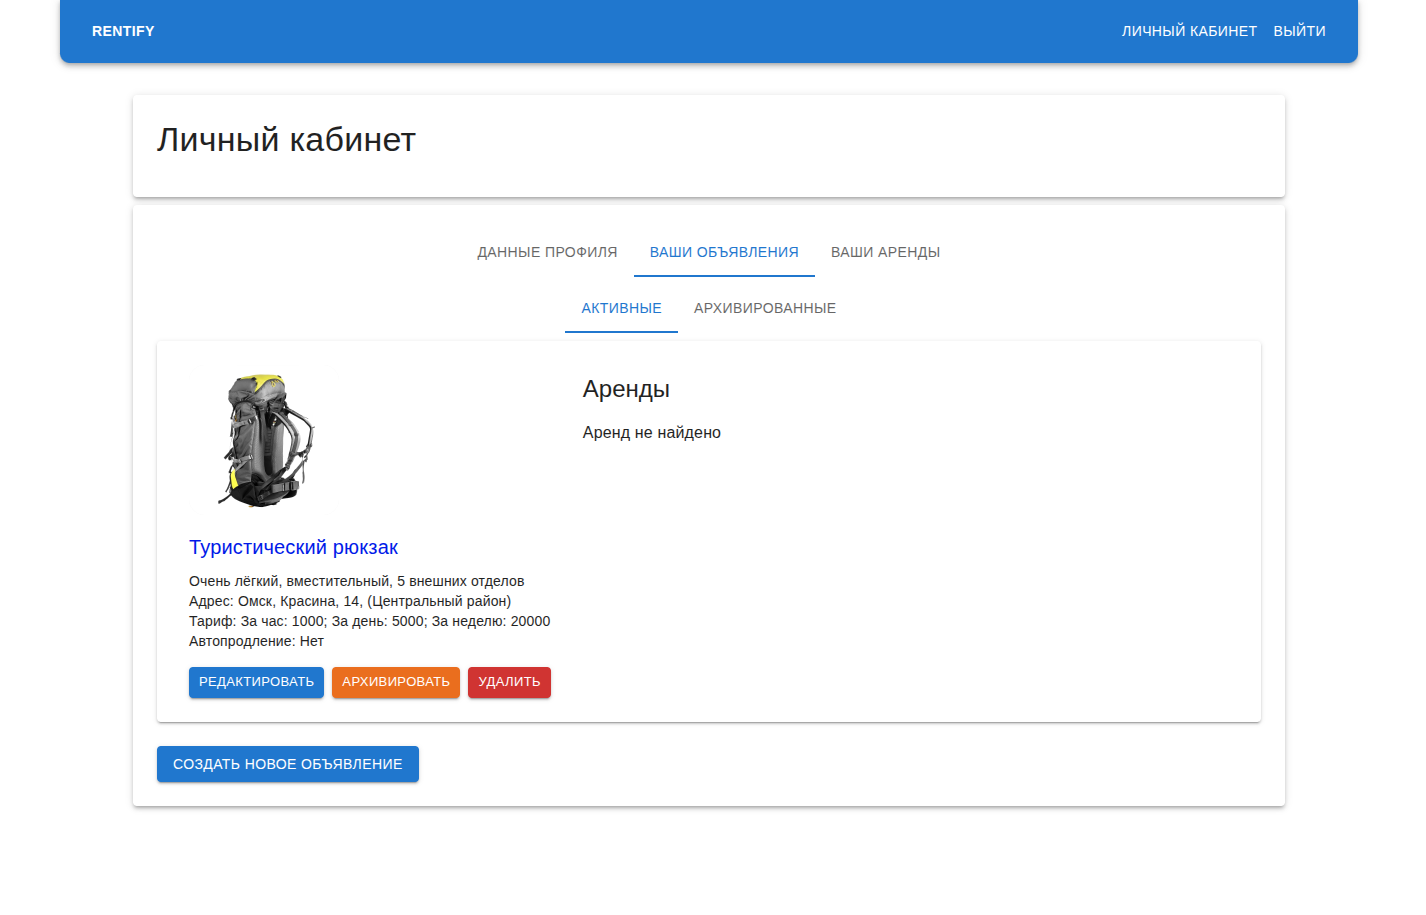
\includegraphics[width=1\textwidth]{listing11.png}
        \end{center}
    \end{frame}

    \begin{frame}
        \begin{center}
            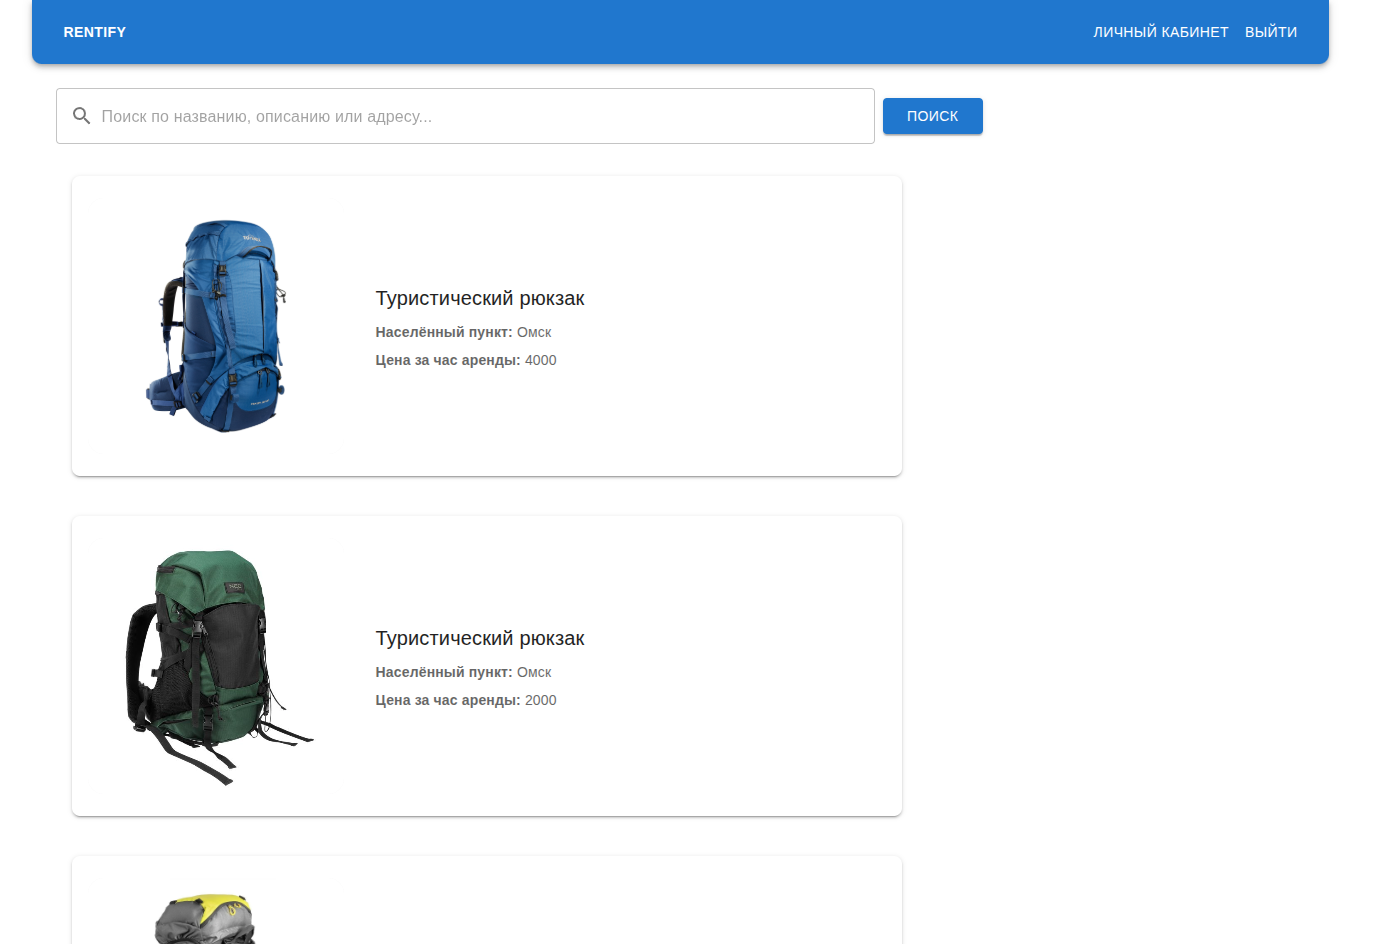
\includegraphics[width=1\textwidth]{search.png}
        \end{center}
    \end{frame}

    \begin{frame}
        \begin{center}
            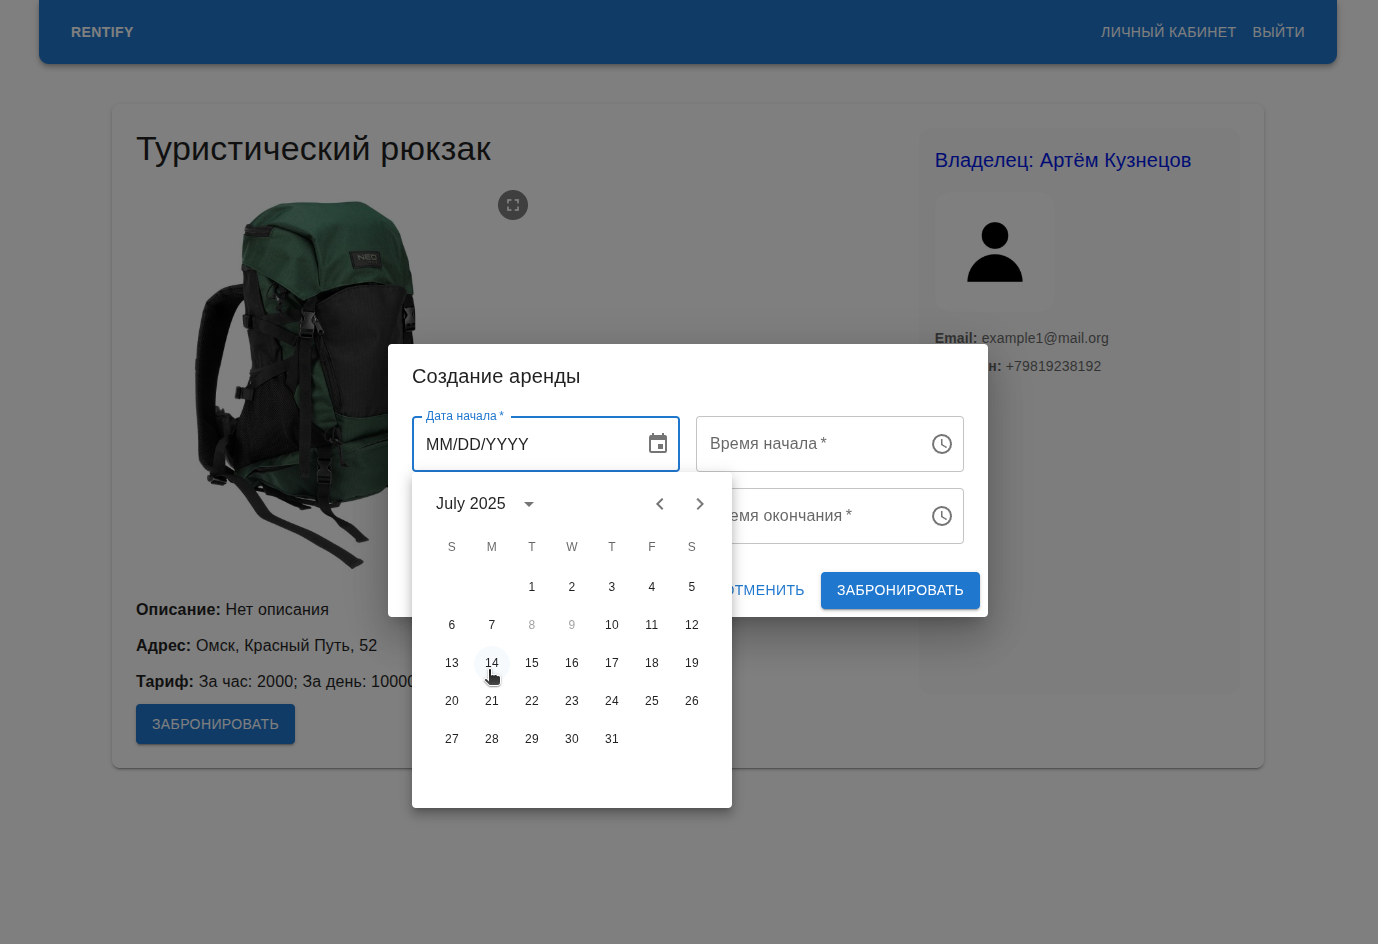
\includegraphics[width=1\textwidth]{booking.png}
        \end{center}
    \end{frame}

    \begin{frame}
        \begin{center}
            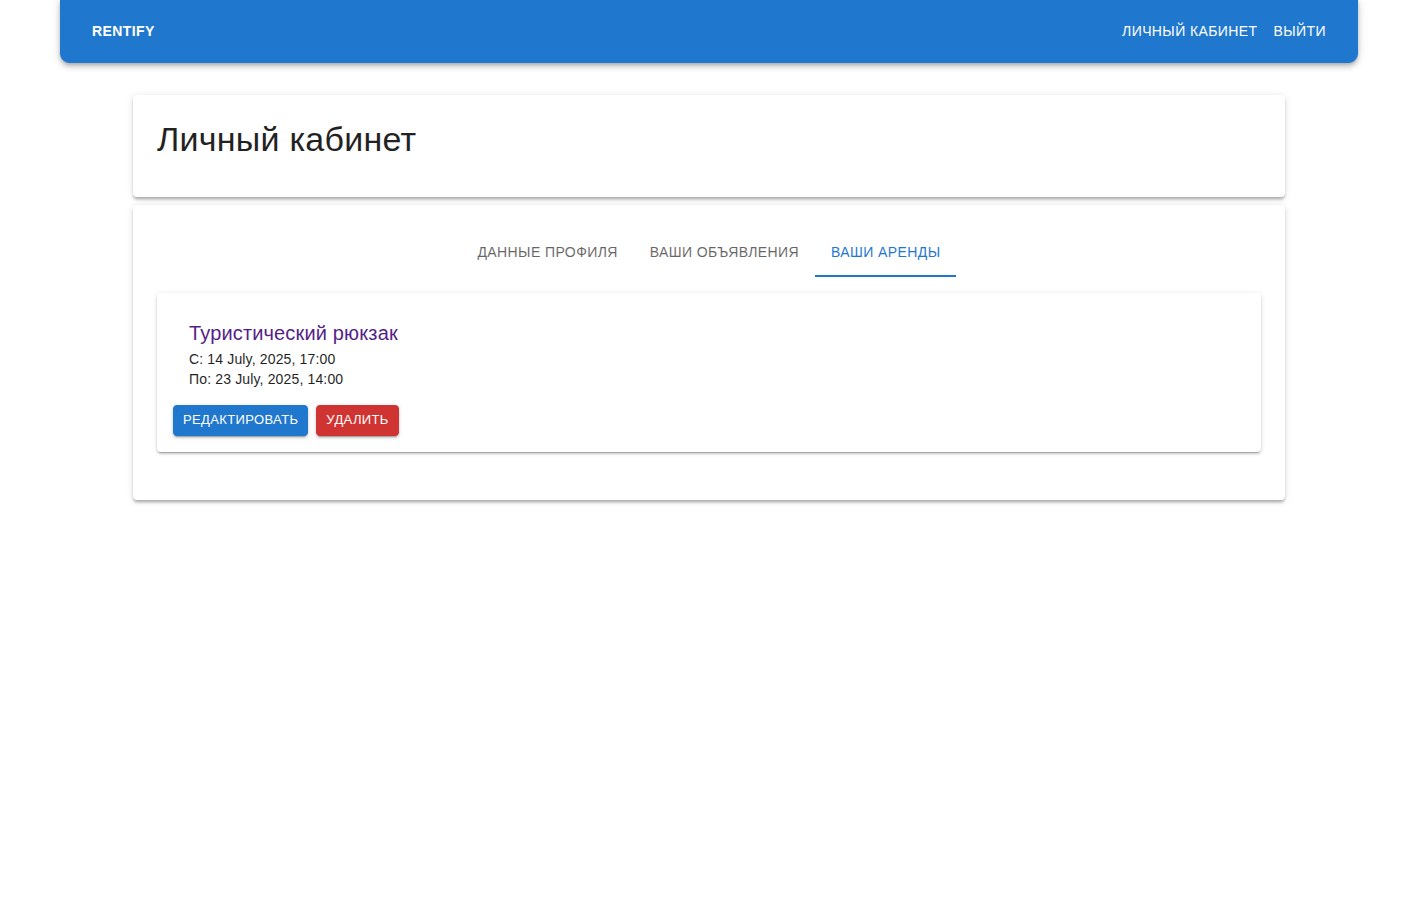
\includegraphics[width=1\textwidth]{booking01.png}
        \end{center}
    \end{frame}

    \begin{frame}
        \begin{center}
            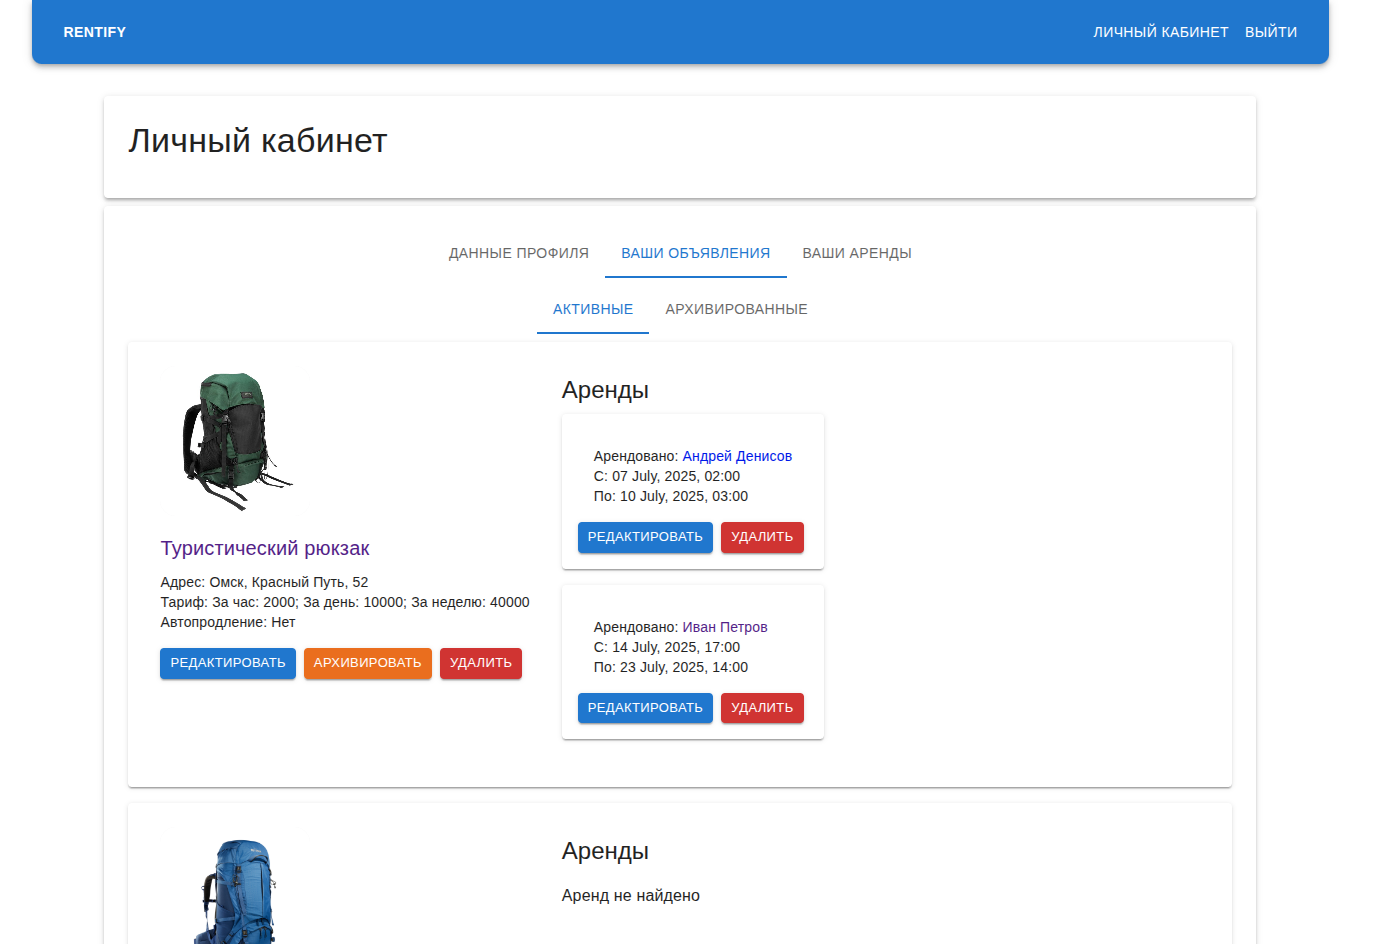
\includegraphics[width=1\textwidth]{listing02.png}
        \end{center}
    \end{frame}
}

\begin{frame}

        \begin{center}
            
\includegraphics[width=0.6\textwidth]{qrcode.png}
        \end{center}
    \end{frame}

\end{document}
